%\rowcolors{0}{lightgray}{darkgray}
%\setlength{\tabcolsep}{6pt}

    \begin{longtable}{|l|p{5.5cm}|p{0.8cm}|p{0.8cm}|p{0.8cm}|p{0.8cm}|p{0.8cm}|p{0.8cm}|p{0.8cm}|p{0.8cm}|p{0.8cm}|p{0.8cm}|p{0.8cm}|}%


\hline
\multicolumn{1}{|c|}{\multirow{2}{*}{ID}} &  \multicolumn{1}{p{5cm}!{\vrule width -1pt}|}{ \multirow{2}{*}{\textbf{Description}}} & \multicolumn{10}{c!{\vrule width -1pt}|}{\textbf{Remaining effort in sprint} (days)}\\  
 \cline{3-12}
 &&   \bfseries 1 & \bfseries 2 & \bfseries3 & \bfseries4 & \bfseries5 & \bfseries6 & \bfseries7 &\bfseries 8 &\bfseries 9 & \bfseries 10\\
\endfirsthead


\multicolumn{12}{c}%
{{\bfseries \tablename\ \thetable{} -- continued from previous page}} \\\hline
\multicolumn{1}{|l!{\vrule width -1pt}|}{ \multirow{2}{*}{\textbf{ID}}} &  \multicolumn{1}{p{5cm}!{\vrule width -1pt}|}{ \multirow{2}{*}{\textbf{Description}}} & \multicolumn{10}{c!{\vrule width -1pt}|}{\textbf{Remaining effort in sprint} (days)}\\  
 \cline{3-12}
   &  & \bfseries 1 & \bfseries 2 & \bfseries3 & \bfseries4 & \bfseries5 & \bfseries6 & \bfseries7 &\bfseries 8 &\bfseries 9 & \bfseries 10
\endhead

 \multicolumn{12}{|c|}{{Continued on next page}} \\ \hline
\endfoot

\endlastfoot
\csvreader[head to column names]{backlog5.csv}{}% use head of csv as column names
 {\\\hline \textbf{\id} & \tasks & \dayone & \daytwo & \daythree & \dayfour & \dayfive  & \daysix & \dayseven & \dayeight & \daynine &\dayten}\\\hline% 
 


\caption{Sprint 5 backlog}
\end{longtable}

\begin{figure}[H]
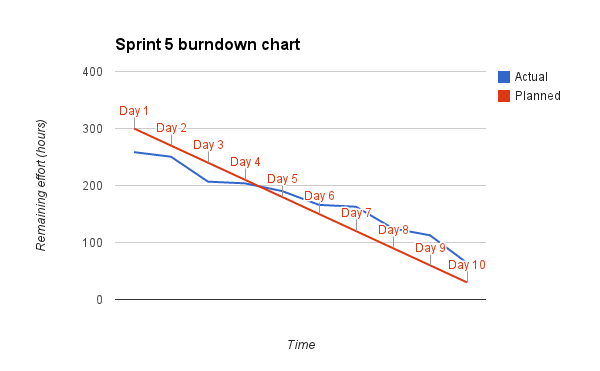
\includegraphics[width=\textwidth]{burndown5.png}
\caption{Burndown chart for sprint 5}
\end{figure}